%\motto{Use the template \emph{chapter.tex} to style the various elements of your chapter content.}
\chapter{Quanteninformationen}
\label{qbits} % Always give a unique label
% use \chaptermark{}
% to alter or adjust the chapter heading in the running head

\chapterauthor{Karin Mustermann, Dominik Neumaier, Thilo Prünte}

\abstract{some abstract}

\section{Der Qubit als Informationsträger}
Die fundamentale Funktionsweise klassischer Computer basiert auf einzelnen Bits, welche jeweils den Zustand $0$ (kein Strom) oder $1$ (Strom) annehmen können. Für Berechnungen werden dann Schaltkreise mit Logikgattern verwendet, die zu einer Ausgabe führen. 
\\

Im Kontext von Quantencomputing ist die kleinste Informationseinheit ein Quantenbit (Qubit). Ein Qubit ist in einer Superposition und kann somit mehr Zustände Annehmen als ein klassisches Bit. 
\section{Praxisbeispiel: Bell-Zustand und Quantenkorrelation}
Bell-Zustände sind spezielle Zustände in der Quantenmechanik, in denen zwei Teilchen maximal miteinander verschränkt sind. Das bedeutet: Ihre Zustände hängen so stark zusammen, dass man sie nicht unabhängig voneinander beschreiben kann – selbst, wenn die Teilchen weit voneinander entfernt sind. Benannt ist der Bell-Zustand nach dem Physiker John S. Bell. Dieser zeigte im Jahre 1964 auf, dass die Vorhersagen der Quantenmechanik im Widerspruch zu den Prinzipien des lokalen Realismus stehen – also der Vorstellung, dass Informationen nicht schneller als Licht übertragen werden können und dass physikalische Größen vor der Messung bereits festgelegt sind. (Vgl. \cite[S.195]{bell_einstein_1964})
\\


Mit der von John S. Bell formulierten Bell-Ungleichung entwickelte Bell ein mathematisches Kriterium, mit dem sich klassische und quantenmechanische Theorien experimentell unterscheiden lassen. Die Quantenmechanik sagt unter bestimmten Bedingungen eine Verletzung dieser Ungleichung voraus. Belegt wurde dies in zahlreichen Experimenten ab 1972, den sogenannten Bell-Test. Seitdem wurde die Verletzung der Bell-Ungleichung in zahlreichen Experimenten mit verschränkten Teilchenpaaren eindeutig nachgewiesen. In allen Fällen bestätigten die Ergebnisse die Vorhersagen der Quantenmechanik. 
(Vgl. \cite[S.53-59]{homeister_quantum_2022})
\\


Insgesamt existieren vier verschiedene Bell-Zustände, die eine Situation maximaler Verschränkung zwischen zwei Qubits beschreiben. Das heißt: Wird der Zustand eines Qubits gemessen, ist das Ergebnis des anderen automatisch bestimmt. Unabhängig von der Entfernung der Qubits voneinander. (Vgl. \cite[S.53-55]{homeister_quantum_2022}) 
\\


Die vier Bell-Zustände sind nachfolgend dargestellt: 
\[
\begin{aligned}
\ket{\Phi^+} &= \frac{1}{\sqrt{2}} (\ket{00} + \ket{11}), \\
\ket{\Phi^-} &= \frac{1}{\sqrt{2}} (\ket{00} - \ket{11}), \\
\ket{\Psi^+} &= \frac{1}{\sqrt{2}} (\ket{01} + \ket{10}), \\
\ket{\Psi^-} &= \frac{1}{\sqrt{2}} (\ket{01} - \ket{10}).
\end{aligned}
\]
\\


Die Erzeugung eines Bell-Zustands basiert auf zwei Schritten. Zu Beginn wird eine Superposition erzeugt, anschließend muss die Verschränkung zwischen den Qubits hergestellt werden. Diese Schritte werden nachfolgend erläutert.
\\


\textbf{Schritt 1 – Superposition erzeugen:} \\
Zuerst wird auf das erste Qubit ein Hadamard-Gatter angewendet. Dadurch wird dieses Qubit in eine Superposition überführt:

\[
\frac{1}{\sqrt{2}} (\ket{0} + \ket{1}) \ket{0} = \frac{1}{\sqrt{2}} (\ket{00} + \ket{10})
\]
\\


\textbf{Schritt 2 – Verschränkung herstellen:} \\
Anschließend folgt ein CNOT-Gatter, bei dem das erste Qubit als Kontroll- und das zweite als Zielqubit fungiert. Dieses Gatter invertiert das Zielqubit nur dann, wenn das Kontrollqubit den Zustand \(\ket{1}\) hat. Dadurch entsteht der Zustand:

\[
\frac{1}{\sqrt{2}} (\ket{00} + \ket{11}) = \ket{\Phi^+}
\]
\\


Es resultiert die vollständige Quantenschaltung zur Erzeugung des Bell-Zustands. Diese ermöglicht es, jeden einfachen Zwei-Qubit-Eingangszustand (\(\ket{00}, \ket{01}, \ket{10}, \ket{11}\)) in einen Bell-Zustand zu überführen.

\[
\Qcircuit @C=1em @R=1em {
\lstick{\ket{0}} & \gate{H} & \ctrl{1} & \qw & \rstick{\frac{1}{\sqrt{2}}(\ket{00} + \ket{11})} \qw \\
\lstick{\ket{0}} & \qw      & \targ    & \qw & \qw
}
\]
\\


Dieser Zustand ist einer der zuvor vorgestellten \textbf{Bell-Zustände} – ein maximal verschränkter Zustand, in dem die Messungen der beiden Qubits perfekt korreliert sind. Wird in einem verschränkten Bell-Zustand das erste Qubit gemessen, so ergibt sich mit gleicher Wahrscheinlichkeit entweder der Zustand \( \ket{0} \) oder \( \ket{1} \). In beiden Fällen legt diese erste Messung sofort auch den Zustand des zweiten Qubits fest: Beobachtet man \( \ket{0} \) am ersten Qubit, ergibt sich insgesamt der Zustand \( \ket{00} \); misst man \( \ket{1} \), resultiert der Zustand \( \ket{11} \). Eine anschließende Messung des zweiten Qubits führt daher zwangsläufig zum gleichen Ergebnis wie beim ersten – entweder beide Qubits liefern 0 oder beide liefern 1. Je nach Eingangs-Zustand und der Reihenfolge der Gatter ergibt sich ein anderer Bell-Zustand. (Vgl. \cite[S.53-54]{homeister_quantum_2022})
\\


Die Eigenschaften von Bell-Zuständen lassen sich mithilfe von Quantencomputern, wie denen von IBM, direkt simulieren und beobachten. In diesem Beispiel wurde ein einfacher Quantenschaltkreis aufgebaut, um einen Bell-Zustand zu erzeugen. Ausgangszustand waren zwei Qubits, die beide den Wert 0 hatten. Zunächst wurde auf das erste Qubit ein Hadamard-Gatter (rotes Gatter) angewendet. Dadurch ging es in eine Überlagerung aus „0“ und „1“ über. Anschließend folgte ein CNOT-Gatter (blaues Gatter), das die beiden Qubits miteinander verschränkte: Wenn das erste Qubit auf „1“ übergeht, kippt das zweite automatisch ebenfalls auf „1“. Das Ergebnis ist ein Zustand, in dem die Qubits perfekt miteinander verbunden sind – man spricht von einem verschränkten Zustand. 

\begin{figure}[h]
    \centering
    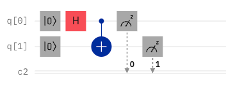
\includegraphics[width=0.4\textwidth]{images/Schaltung_IBM.png}
    \caption{Quantenschaltung - IBM Quantum Learning Platform.}
    \label{fig:meinbild}
\end{figure}

Nach dem Aufbau der Schaltung wurden auf dem IBM-Quantencomputer Messungen durchgeführt. Das bedeutet, dass die Qubits im Z-Basiszustand ausgelesen werden um zu überprüfen, ob sie im Zustand „0“ oder „1“ sind. 

\begin{figure}[h]
    \centering
    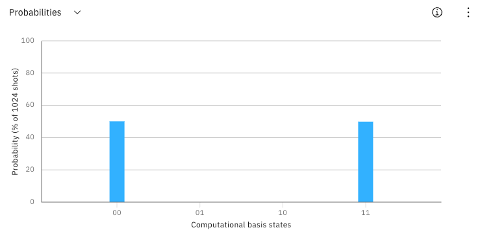
\includegraphics[width=0.6\textwidth]{images/results_ibm.png}
    \caption{Wahrscheinlichkeitsverteilung - IBM Quantum Learning Platform.}
    \label{fig:meinbild}
\end{figure}


Wie das Histogramm zeigt, wurden ausschließlich die Zustände „00“ und „11“ beobachtet - und zwar mit jeweils rund 50\% Wahrscheinlichkeit. Die Zustände „01“ oder „10“, bei denen sich die beiden Qubits unterscheiden würden, traten gar nicht auf. Dies ist ein typisches Verhalten eines Bell-Zustands und belegt, dass die Qubits verschränkt sind. Bemerkenswert ist dabei: Diese Quantenkorrelation bleibt bestehen, selbst wenn die Qubits räumlich voneinander getrennt wären. Die Messergebnisse des einen beeinflussen scheinbar sofort das andere – ein Verhalten, das mit klassischer Physik nicht erklärbar ist. (Vgl. \cite{Bell State ZZ-Measurement}) 
\\


Ein anschauliches Beispiel für die Eigenschaften verschränkter Zustände liefert auch ein Gedankenexperiment mit zwei beispielhaften Personen, Alice und Bob. Angenommen die beiden erzeugen gemeinsam entsprechend der vorhergehenden Ausführungen folgenden Bell-Zustand:
\[
\frac{1}{\sqrt{2}} (|00\rangle + |11\rangle).
\]
Alice erhält nun das erste Qubit, Bob das zweite Qubit. Angenommen die beiden befinden sich ursprünglich in einem Haus im gleichen Raum. Bob nimmt nun sein Qubit mit in ein anderes Zimmer. Solange keine Messung erfolgt und die Qubits vor äußeren Einflüssen geschützt sind, bleibt die Verschränkung erhalten – unabhängig von der räumlichen Trennung. Führt nun einer der beiden eine Messung durch, so ist das Ergebnis zufällig: Mit einer Wahrscheinlichkeit von 50\,\% wird $|0\rangle$ gemessen, mit 50\,\% $|1\rangle$. Erst wenn Alice und Bob ihre Ergebnisse miteinander vergleichen, zeigt sich die Besonderheit: Ihre Messergebnisse stimmen stets überein. Es resultiert eine perfekte Korrelation, unabhängig von Raum und Zeit. (Vgl. \cite[S.54]{homeister_quantum_2022})
\\


Genau darin zeigt sich der Informationsgehalt eines verschränkten Zustands: Die Information liegt nicht in einem einzelnen Qubit, sondern nur in ihrer gemeinsamen Beziehung. Diese Simulation macht das abstrakte Konzept der Quantenverschränkung greifbar und bietet einen intuitiven Zugang zu den Grundlagen der Quanteninformation. Es zeigt anschaulich, wie Quantencomputer fundamentale Prinzipien der Quantenmechanik sichtbar und messbar machen. 
\printbibliography
